This internship was particular in two ways: first the university of Leiden was not accostumed to the type of work I was proposing. Internship of this type were unheard of, and I was also providing them with a research subject. I worked under the supervision of M. Verschoof-van der Vaart, a PhD candidate in the department of Digital Archaeology of Leiden University. M. Verschoof-van der Vaart is also working on automated detection in \gls{lidar}.

Then the COVID-19 situation profoundly modified planning. Initially, I was planned to stay at Leiden in the Netherlands, and work physically within the University, in a lab made for Master students. The COVID-19 forced the university to close down shortly before my departure, and then France entered a two month quarantine. This modified the way I was going to work.  

Under those unique circumstances, I was allowed a rare freedom, and much trust. I was lucky enough that I could conduct my work remotely, since most of it was writing documents, studying and reading papers, training and evaluating networks. 

I spent the entire internship working from home. I would interact regularly with Leiden University to give updates or give reports. I used the computing server of my old computer club, the DTRE to train the networks and run experiments.

However this situation also came with negative consequences. Since I was not physically present at the University, frequent, non formal contact was not possible. I also had issues gaining access to the computing facilities of the University, which slowed my work by forcing me to use a less performant computing server. Due to this, I had to severely restrict the reach of this research project. I was planning to give a serious look at the improvements and other study paths presented in Section~\ref{upgrades}, but due to a lack of time and computing capabilities, I could not. 

I first proposed a study schedule to my advisor, reproduced as a GANTT in Figure~\ref{fig:gantt}, splitting my 6 months supposed stay into different sections. The first section of the project was a thorough state of the art review of satellite detection techniques, with a write up on each article, along with a detailed planning and recommendation on the architecture and training of the model, which a synthetic version is presented in Section~\ref{sota} and Section~\ref{yolo}. Then came the actual training of the model, and continuous improvements. Finally, a significant amount of time was reserved for the redaction of this present document.  

\begin{figure}
  \centering
	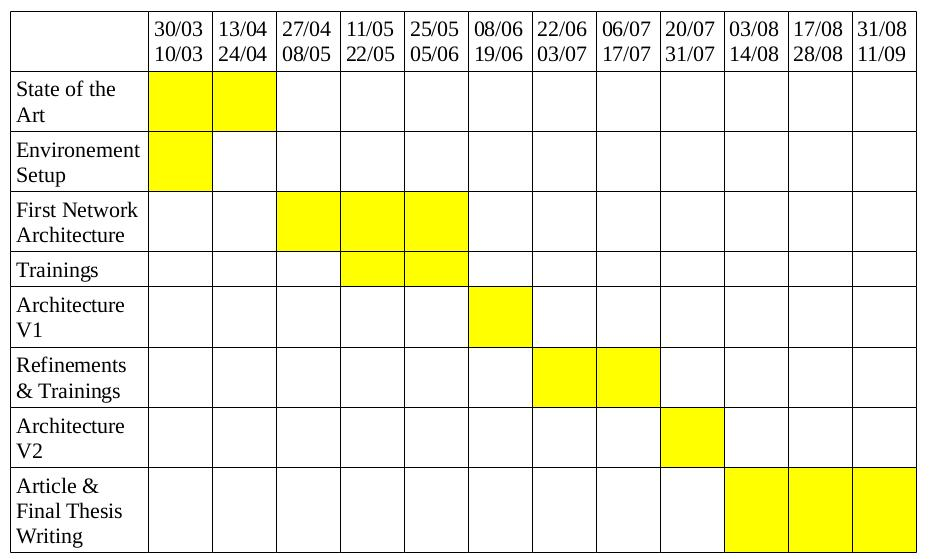
\includegraphics[width=\textwidth]{gantt.jpg}
	\caption[]{Initial GANTT for the study project}
  \label{fig:gantt}
\end{figure}

Splitting my time between coding tools, training and evaluating networks and redacting documents was a challenging task. Since I was in charge of my planning, and how my day was going to be spent, I needed to make sure that all my tasks were done before I could move on to the next phase. While the independance I was given meant I had entire freedom on how I would accomplish my tasks and when, it also meant I had to work on my organisational skills, and make sure I did not do superfluous work. 

Luckily, training networks to completion took a fairly long time. This meant that I could use this time to advance myself on other tasks, such as redacting reports, or programmation. This multitasking was key in the completion of this project in due time. On a typical day I would first check on the results of a training launched the previous day. I would then report those results on a file, along with some identifying informations, such as the day or the name of the network configuration file. I would then start another training, and use the time left to write my thesis, or compute some metrics. 
